\documentclass[12pt, a4paper, twoside]{article}
\usepackage[utf8]{inputenc}
\usepackage{graphicx}
\graphicspath{ {images/} }
\PassOptionsToPackage{hyphens}{url}
\usepackage{hyperref}
 
\title{Vibration of a Rotating Cantilever Beam}
\author{Süleyman Muti}
\date{May 19, 2020}

\begin{document}


\maketitle


\begin{abstract}
	
This study demonstrates the natural frequency analysis of a cantilever beam subjected to centrifugal loading. This is analogous to the vibrations of compressor and turbine blades.

The free and open-source finite element analysis software CalculiX is used \cite{CalculiX_website}.

\end{abstract}


\section{Description}

The beam is built into a rigid disk of $r$ $mm$ radius, rotating about its axis at a speed of $\Omega$ $rpm$. It is $\ell$ $mm$ long, $w$ $mm$ wide, $t$ $mm$ thick, and makes an angle of $\alpha$ $degrees$ with the rotation axis, as shown in Figure ~\ref{fig:rotating_cantilever_beam}.

The plate is made of steel, with a Young's modulus $2.17 \times 10^{5}$ $MPa$ and a density of $7.85 \times 10^{-9}$ $tonne/mm^3$.

\begin{figure}[h]
    \centering
    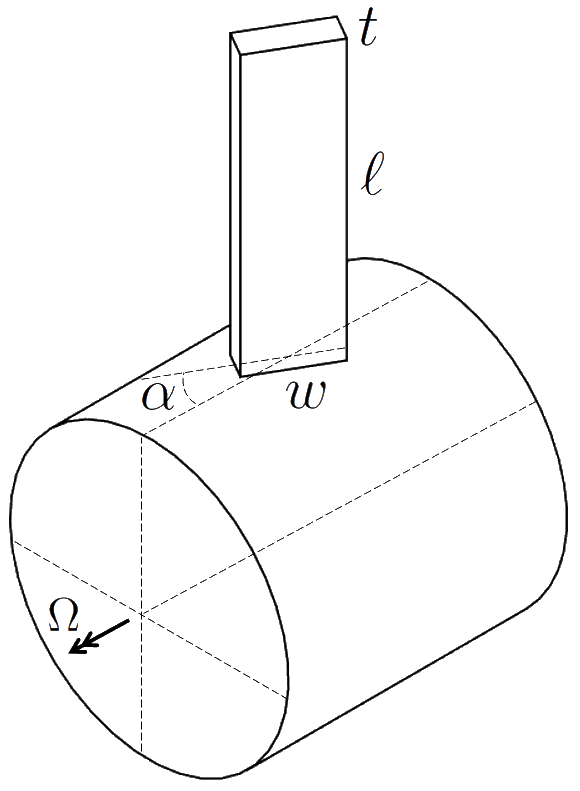
\includegraphics[scale=0.5]{rotating_cantilever_beam}
    \caption{Rotating cantilever beam.}
    \label{fig:rotating_cantilever_beam}
\end{figure}


\section{Pre-processing}
Dimensions are given below:

$r$ $=$ $150$ $mm$,

$\ell$ $=$ $328$ $mm$,

$w$ $=$ $28$ $mm$,

$t$ $=$ $3$ $mm$,

$\alpha$ $=$ $0$ $degrees$.

The general purpose quadratic brick element with reduced integration (C3D20R) is used. See Figure ~\ref{fig:pre} for the finite element model of the rotating cantilever beam. The the beam is cantilevered at $r$ $=$ $150$ $mm$. A rotational speed of $\Omega$ $=$ $4500$ $rpm$ about the axis of the rigid disk is applied to the whole model.

\begin{figure}[h]
	\centering
	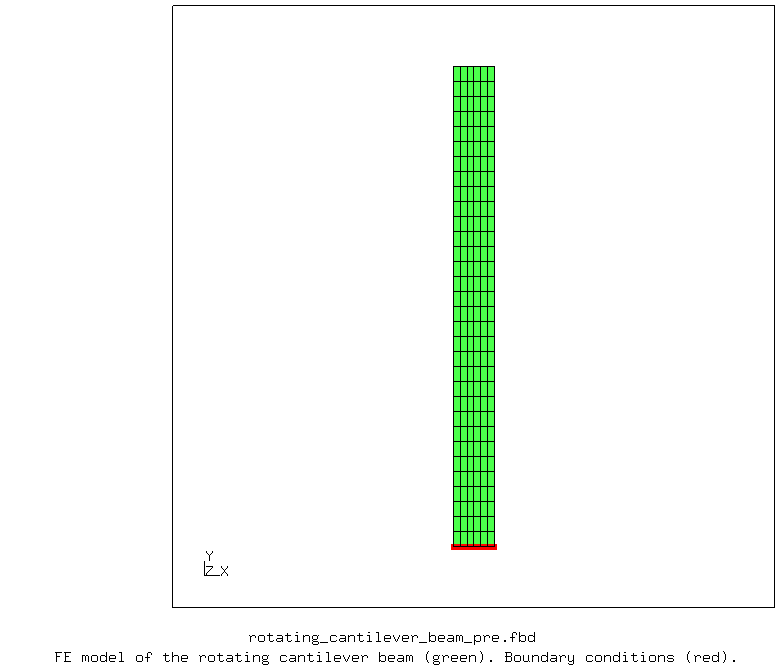
\includegraphics[scale=0.5]{pre}
	\caption{Finite element model of the rotating cantilever beam.}
	\label{fig:pre}
\end{figure}


\section{Results}

The first vibration mode is obtained as $71.81$ $Hz$ from CalculiX. This result is can be compared with the results reported for Abaqus 6.6 in Reference \cite{abaqus_manual}. Table ~\ref{table:freqs} lists the first three modes obtained with CalculiX.


\begin{figure}[h]
	\centering
	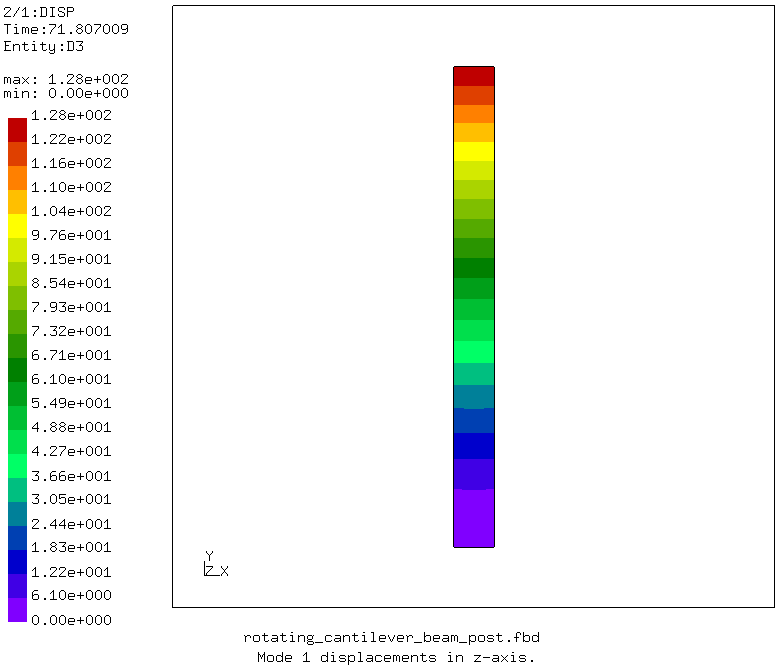
\includegraphics[scale=0.5]{post}
	\caption{Mode 1 displacements in z-axis.}
	\label{fig:post}
\end{figure}


\begin{table}[ht]
	\caption{Natural frequencies of the rotating cantilever beam.}% title of Table
	\centering % used for centering table
	\begin{tabular}{c c}% centered columns (4 columns)
		\hline\hline                        %inserts double horizontal lines
		Mode \# & Frequency $[Hz]$ \\ [0.5ex]% inserts table
		%heading
		\hline\hline                 % inserts single horizontal line
		1 & 71.807009 \\% inserting body of the table
		2 & 243.222157 \\
		3 & 273.155573 \\[1ex]      % [1ex] adds vertical space
		\hline%inserts single line
	\end{tabular}
	\label{table:freqs}% is used to refer this table in the text
\end{table}


\clearpage
% Bibliographic references
\begin{thebibliography}{9}
	
\bibitem{CalculiX_website} 
CalculiX, A Free Software Three-Dimensional Structural Finite Element Program. \url{http://www.calculix.de/}


\bibitem{abaqus_manual} 
Washington University in St. Louis, ABAQUS Benchmarks Manual, Vibration of a rotating cantilever plate. \url{https://classes.engineering.wustl.edu/2009/spring/mase5513/abaqus/docs/v6.6/books/bmk/default.htm?startat=ch01s04ach43.html}

\end{thebibliography}


\end{document}